\documentclass[11pt]{article}

% ============================================================
% Packages
% ============================================================

\usepackage[margin=1in]{geometry}

\usepackage{graphicx}
\usepackage{amsmath}
\usepackage{amssymb}
\usepackage{booktabs}
\usepackage{multirow}
\usepackage{array}
\usepackage{enumitem}
\usepackage{hyperref}
\usepackage{xcolor}
\usepackage{float}
\usepackage{natbib}
\usepackage{tcolorbox}

\tcbuselibrary{skins,breakable}

\hypersetup{
    colorlinks=true,
    linkcolor=blue,
    citecolor=blue,
    urlcolor=blue
}

\newtcolorbox{highlightbox}{
    colback=gray!5,
    colframe=black!60,
    boxrule=0.5pt,
    arc=2pt,
    left=6pt,
    right=6pt,
    top=4pt,
    bottom=4pt
}

% ============================================================
% Title
% ============================================================

\title{
\textbf{
Beyond Fixed Directions:\\
Representational Geometry of Reasoning and Memorization in Large Language Models
}
}

\author{
Shaheen Nabi\\
Indian Institute of Science (IISc), Bangalore\\
\texttt{devshaheen0@gmail.com}
}

\date{August 2026}

% ============================================================

\begin{document}

\maketitle

\begingroup
\renewcommand\thefootnote{}
\footnotetext{
Code, configs, and checkpoints (where feasible) will be released at:
\url{https://github.com/PLACEHOLDER/repo}.
}
\endgroup

% ============================================================


\begin{abstract}

We study whether reasoning-oriented and factual-recall task representations in Qwen3-0.6B are linearly separable, and whether the observed separation can be captured by a single direction in hidden representation space. Initial MATH-500 versus PopQA experiments showed perfect final-layer probing performance, but prompt token length alone predicted the label with 96.5\% accuracy and 0.994 AUROC. A strict length-matched follow-up preserved hidden-state separability but produced only 10 examples per class. We therefore constructed an expanded controlled dataset with 200 reasoning-oriented examples from MATH-500/GSM8K and 200 factual-recall examples from PopQA/TriviaQA. On this dataset, length-only performance dropped to \(0.6475 \pm 0.0533\) accuracy and \(0.6645 \pm 0.0585\) AUROC, while a TF--IDF lexical baseline remained strong at \(0.9600 \pm 0.0146\) accuracy and \(0.9911 \pm 0.0113\) AUROC. In the final RQ1 experiment, we directly tested one-dimensional directions at all 28 transformer layers using held-out cross-validation. A mean-difference direction reaches \(1.0000 \pm 0.0000\) AUROC at layer 18, and a normalized logistic-probe direction reaches \(1.0000 \pm 0.0000\) AUROC at layer 12, matching the full 1024-D linear probe. These results provide strong support for an approximately single-direction separation of the studied task groups, while lexical and domain confounds prevent a stronger causal or semantic claim about reasoning itself.

\end{abstract}

\begin{highlightbox}
\textbf{Key findings}

\begin{itemize}[leftmargin=*]
    \item The original MATH-500 versus PopQA separation was strongly confounded by prompt length, so the first perfect probe result was diagnostic rather than conclusive.
    \item The expanded 400-example control reduced length as a dominant predictor, but TF--IDF lexical features remained highly predictive.
    \item The final RQ1 single-direction test shows that one scalar projection is sufficient to match the full 1024-D linear probe on the current controlled task groups.
    \item The best mean-difference direction occurs at layer 18 and achieves \(0.9975 \pm 0.0050\) accuracy and \(1.0000 \pm 0.0000\) AUROC.
    \item The best probe-weight direction occurs at layer 12 and also achieves \(0.9975 \pm 0.0050\) accuracy and \(1.0000 \pm 0.0000\) AUROC.
    \item RQ1 receives strong support for an approximately single-direction task-group separation, but not for a causal or intrinsic reasoning mechanism.
\end{itemize}

\end{highlightbox}

\section{Introduction}\section{Introduction}

Recent work increasingly analyzes high-level model behaviors through
geometric structure in activation space. If a behavior corresponds to
a simple direction, then it may be possible to measure, compare, or
intervene on that behavior using a compact linear object. This
possibility is especially attractive for reasoning and factual recall,
two capabilities that are central to the behavior of modern language
models.

However, apparent linear separation between two behavioral categories
does not by itself imply that a model represents the underlying
concepts along a single semantic direction. In probing experiments,
the labels of interest are often correlated with source dataset,
prompt length, lexical content, domain, formatting, and other surface
properties. A linear classifier can exploit these artifacts while
appearing to decode a high-level concept.

This paper studies this issue in the setting of reasoning-oriented
versus factual-recall tasks. We ask whether these task groups can be
separated in Qwen3-0.6B's hidden representation space, and whether any
observed separation survives progressively stronger controls.

Our initial diagnostic experiment compared MATH-500 against PopQA.
The result was superficially strong: final-layer PCA separated the two
datasets and a linear probe achieved perfect 5-fold classification.
But a length-only baseline also predicted the label with 96.5\%
accuracy, showing that the initial result was strongly confounded. A
strict pairwise length-matched experiment reduced this confound, but
only yielded a 20-example dataset.

The current expanded experiment therefore uses four datasets:
MATH-500 and GSM8K for reasoning-oriented tasks, and PopQA and TriviaQA
for factual recall. We deduplicate examples, apply a common prompt
template, measure token length using the custom Qwen3 tokenizer, and
construct a distributionally length-matched 400-example dataset. This
larger control shows that Qwen final-layer representations remain
almost perfectly separable after substantial length control. At the
same time, a simple TF--IDF baseline remains highly predictive,
indicating that lexical and domain cues still explain much of the task
distinction.

The main contribution of the current draft is therefore diagnostic and
methodological. We show that representation-level separation is robust
to a stronger token-length control, but also that strong linear
separability is not yet evidence of a single reasoning direction.
Additional controls are required before making that stronger claim.

% ============================================================

\section{Problem Formulation}

We investigate the representational geometry of reasoning and
memorization in large language models.

Given a language model

\[
f_{\theta},
\]

we extract hidden representations

\[
h^{(l)} \in \mathbb{R}^{d}
\]

from transformer layer \(l\), where \(d\) denotes the hidden
dimension.

Our central question is whether reasoning and memorization can be
adequately characterized by a single linear direction in
representation space, or whether their distinction requires richer
multidimensional structure.

A central methodological challenge is that behavioral labels can be
correlated with simple dataset properties. Consequently, linear
separability alone is insufficient evidence for a semantic
reasoning--memorization direction.

We therefore distinguish between three questions:

\begin{enumerate}

    \item Are reasoning and memorization datasets linearly separable
    from hidden representations?

    \item Does this separation remain after controlling for observable
    dataset artifacts such as prompt length and formatting?

    \item If controlled separation remains, can it be adequately
    represented by a single direction, or does it require a
    multidimensional subspace?

\end{enumerate}

More broadly, we investigate:

\begin{itemize}

    \item whether reasoning and memorization are linearly separable
    across transformer depth;

    \item whether a single direction is sufficient to characterize
    this separation;

    \item how these representations evolve during reinforcement
    learning;

    \item whether identified representational structures generalize
    across tasks and datasets;

    \item and whether reasoning and memorization consist of multiple
    interpretable latent components.

\end{itemize}

Our framework consists of four complementary analyses, treated as
research questions RQ1--RQ4.

% ============================================================

\section{RQ1: Linear Structure of Reasoning and Memorization}

\subsection{Research Question}

We first ask:

\begin{quote}
\textit{Can reasoning and memorization be represented by a single
linear direction in the model's hidden representation space?}
\end{quote}

A strong single-direction hypothesis predicts that the relevant
reasoning--memorization signal can be captured primarily through one
axis in representation space.

A multidimensional hypothesis instead predicts that multiple
independent directions are required to characterize the distinction.

Importantly, neither PCA separation nor high linear-probe accuracy is
by itself sufficient to establish the single-direction hypothesis.
Both can arise from dataset-level confounds.

% ------------------------------------------------------------

\subsection{Initial Experimental Setup}

\paragraph{Model.}

Our initial experiments use Qwen3-0.6B, consisting of 28 transformer
layers with hidden dimension

\[
d = 1024.
\]

Larger models will be considered in subsequent validation experiments.

\paragraph{Initial datasets.}

For the initial diagnostic experiment, we construct a balanced binary
dataset containing:

\begin{itemize}

    \item 100 reasoning examples sampled from MATH-500;

    \item 100 factual-recall / memorization examples sampled from
    PopQA.

\end{itemize}

The resulting dataset contains

\[
N = 200
\]

examples.

Each example retains metadata including its identifier, source
dataset, behavioral label, and original problem or question.

This initial dataset is intentionally treated as a diagnostic setup
rather than a final controlled benchmark because source dataset and
behavioral label are perfectly correlated:

\[
\text{MATH-500} \rightarrow \text{reasoning},
\]

\[
\text{PopQA} \rightarrow \text{memorization}.
\]

% ------------------------------------------------------------

\subsection{Representation Extraction}

For each prompt, we perform a forward pass through the complete
transformer without autoregressive generation.

At each transformer block \(l\), we extract the residual-stream
representation corresponding to the final token position of the
formatted prompt:

\[
h_i^{(l)}
=
H_i^{(l)}[-1],
\]

where

\[
H_i^{(l)}
\in
\mathbb{R}^{T_i \times d}
\]

contains the hidden representations of all prompt positions after
transformer block \(l\).

The extracted position corresponds to the final token of the complete
formatted prompt supplied to the model before generation. It is
therefore not necessarily the final semantic token of the original
question.

Representations are collected immediately after each transformer
block and before the final RMS normalization and language-model head.

For each example, this produces

\[
H_i
\in
\mathbb{R}^{28 \times 1024}.
\]

Stacking examples produces

\[
H_R
\in
\mathbb{R}^{100 \times 28 \times 1024}
\]

for reasoning and

\[
H_M
\in
\mathbb{R}^{100 \times 28 \times 1024}
\]

for memorization.

Extraction is performed in evaluation mode without gradient
computation or autoregressive KV-cache generation.

% ------------------------------------------------------------

\subsection{Layer-wise Representation Construction}

Because representations evolve through transformer depth, each layer
is analyzed independently.

For layer \(l\), we define

\[
R^{(l)}
\in
\mathbb{R}^{100 \times 1024}
\]

and

\[
M^{(l)}
\in
\mathbb{R}^{100 \times 1024}.
\]

They are concatenated as

\[
X^{(l)}
=
\begin{bmatrix}
R^{(l)} \\
M^{(l)}
\end{bmatrix}
\in
\mathbb{R}^{200 \times 1024}.
\]

The labels are

\[
y_i =
\begin{cases}
1, & \text{reasoning},\\
0, & \text{memorization}.
\end{cases}
\]

The initial experiments reported below analyze only the final
transformer layer.

% ============================================================

\subsection{Initial PCA Analysis}

We first apply Principal Component Analysis (PCA) to the final-layer
representation matrix

\[
X^{(28)}
\in
\mathbb{R}^{200 \times 1024}.
\]

PCA is unsupervised: the reasoning and memorization labels are not
provided during fitting.

The first principal component

\[
v_1 \in \mathbb{R}^{1024}
\]

captures the direction of maximum variance among the representations.
The second component \(v_2\) captures the largest remaining variance
subject to orthogonality with \(v_1\).

For representation \(h_i\), its coordinates are

\[
z_{i1}
=
(h_i-\mu)^\top v_1
\]

and

\[
z_{i2}
=
(h_i-\mu)^\top v_2,
\]

where \(\mu\) is the mean representation across all 200 examples.

Labels are applied only after PCA in order to visualize how the
behavioral categories align with the discovered geometry.

% ------------------------------------------------------------

\subsection{Initial PCA Results}

On the final transformer layer, PC1 explains

\[
49.04\%
\]

of total representation variance and PC2 explains

\[
8.88\%.
\]

Together,

\[
\mathrm{Var}(PC1,PC2)=57.92\%.
\]

The resulting projection exhibits strong visual separation between
the MATH-500 reasoning examples and PopQA memorization examples,
primarily along PC1.

\begin{figure}[H]
    \centering

    % Replace with actual figure:
    %
    % \includegraphics[
    % width=0.75\textwidth
    % ]{figures/final_layer_pca.png}

    \fbox{
        \parbox[c][5cm][c]{0.75\textwidth}{
            \centering
            Final-layer PCA figure placeholder
        }
    }

    \caption{
    PCA projection of final-layer hidden representations for 100
    MATH-500 reasoning examples and 100 PopQA memorization examples.
    PC1 explains 49.04\% of total variance and PC2 explains 8.88\%.
    Behavioral labels are used only to color the resulting PCA
    coordinates and are not provided during PCA fitting.
    }

    \label{fig:initial-pca}

\end{figure}

At this stage, this result establishes only that source/behavioral
labels align strongly with a dominant axis of variation in the
final-layer representation space.

It does not establish that PC1 specifically encodes reasoning versus
memorization.

% ============================================================

\subsection{Initial Linear-Probe Experiment}

We next test whether the binary label can be linearly decoded from the
final-layer hidden representations.

We train an L2-regularized logistic-regression probe of the form

\[
p(y=1\mid h)
=
\sigma(w^\top h+b).
\]

Unlike PCA, the linear probe explicitly receives reasoning and
memorization labels during training.

We first perform a preliminary stratified train--test split with 160
training examples and 40 held-out examples.

The probe achieves

\[
\mathrm{Accuracy}=1.00.
\]

We subsequently evaluate the probe using 5-fold stratified
cross-validation. Each fold contains 160 training examples and 40
held-out examples while preserving the class balance.

Across all five folds, we observe

\[
\mathrm{Accuracy}
=
1.000 \pm 0.000,
\]

\[
\mathrm{Balanced\ Accuracy}
=
1.000 \pm 0.000,
\]

and

\[
\mathrm{AUROC}
=
1.000 \pm 0.000.
\]

Thus, under random within-dataset cross-validation, the MATH-500 versus
PopQA label is perfectly linearly decodable from the final-layer
representations.

However, this result does not establish that the probe has learned a
semantic reasoning--memorization distinction. Because source dataset
and behavioral label are perfectly correlated, the probe may instead
exploit dataset-specific properties.

% ============================================================

\subsection{Diagnostic Controls}

The unexpectedly perfect probe performance motivates a series of
diagnostic controls designed to test whether simple dataset artifacts
can explain the observed separation.

% ------------------------------------------------------------

\subsubsection{Random-Label Control}

We randomly permute the reasoning and memorization labels while
preserving the hidden representations and repeat the probing
procedure.

Performance falls to approximately chance-level behavior.

This provides evidence that the probing implementation itself is not
trivially producing perfect classification independent of the labels.

% ------------------------------------------------------------

\subsubsection{Prompt-Format Control}

Inspection of tokenized prompts reveals substantial formatting
differences between the original reasoning and memorization inputs.

We therefore normalize the prompt wrapper so that both classes use the
same input formatting and re-extract the hidden representations.

After prompt-format normalization, the hidden-state linear probe still
achieves perfect classification:

\[
\mathrm{Accuracy}=1.00,
\]

with corresponding perfect balanced accuracy and AUROC.

Therefore prompt-wrapper differences alone do not explain the
observed separation.

% ------------------------------------------------------------

\subsubsection{Token-Length Baseline}

Inspection of the tokenized inputs also reveals a substantial
difference in prompt lengths between the two classes, with MATH-500
reasoning prompts generally being considerably longer than PopQA
questions.

To quantify whether this simple scalar feature predicts the class
label, we train a baseline classifier using only prompt token length.

Despite receiving no hidden representations, the length-only
classifier achieves approximately

\[
\mathrm{Accuracy}\approx0.965
\]

and

\[
\mathrm{AUROC}\approx0.994.
\]

This is a critical diagnostic result.

A single surface-level feature---prompt token length---is sufficient
to predict the reasoning versus memorization dataset label with very
high accuracy.

Consequently, the perfect hidden-state probe cannot currently be
interpreted as evidence for an intrinsic reasoning--memorization
representation.

% ============================================================

\subsection{Interpretation of the Initial Experiment}

The initial PCA and probing experiments demonstrate that MATH-500 and
PopQA are strongly distinguishable in Qwen3-0.6B's final-layer
representation space.

However, the diagnostic controls reveal that the experimental labels
are strongly confounded with dataset-level properties.

In particular:

\begin{itemize}

    \item PCA exhibits strong unsupervised separation, but PCA does not
    identify the semantic cause of this separation;

    \item the final-layer linear probe achieves perfect 5-fold
    cross-validation performance;

    \item random-label performance falls to approximately chance,
    indicating that the evaluation pipeline is functioning as
    expected;

    \item standardizing the prompt wrapper does not eliminate the
    perfect hidden-state separation;

    \item token length alone predicts the class label with
    approximately 96.5\% accuracy and 0.994 AUROC.

\end{itemize}

These results indicate that the original experiment is not a clean
test of the single-direction hypothesis.

Specifically, the observed representation geometry may reflect a
mixture of:

\begin{itemize}

    \item reasoning versus factual recall;

    \item prompt length;

    \item mathematical versus factual language;

    \item lexical structure;

    \item task domain;

    \item and source-dataset identity.

\end{itemize}

We therefore treat the initial MATH-500 versus PopQA experiment as a
\textbf{diagnostic experiment} rather than evidence for a semantic
reasoning--memorization direction.

% ============================================================

\subsection{Controlled Experimental Design}

The next stage of RQ1 is designed to separate reasoning--memorization
structure from dataset artifacts.

% ------------------------------------------------------------

\subsubsection{Length-Matched Evaluation: Design}

We first construct matched subsets of reasoning and memorization
examples with comparable token-length distributions.

For reasoning example \(r_i\) and memorization example \(m_j\), we
seek pairs satisfying

\[
|L(r_i)-L(m_j)| \leq \delta,
\]

where \(L(\cdot)\) denotes tokenized prompt length and \(\delta\)
controls the matching tolerance.

Before interpreting hidden-state results, we require the length-only
baseline to fall substantially toward chance performance on the
matched dataset.

We then repeat:

\begin{itemize}

    \item PCA;

    \item linear probing;

    \item random-label control;

    \item and representation analysis.

\end{itemize}

This experiment tests how much of the original separation survives
after controlling the strongest identified scalar confound.

% ------------------------------------------------------------

\subsubsection{Length-Matched Evaluation: Results}

We run the length-matched control using the same Qwen3 tokenizer and
the same prompt-tokenization pipeline used for representation
extraction. We set

\[
\delta = 5
\]

tokens and perform one-to-one matching without replacement. Full
100-vs-100 matching is not possible under this tolerance. The maximum
balanced matched subset contains

\[
N_R = 10,\qquad N_M = 10,
\]

for a total of 20 examples.

The matched hidden-state tensors have the expected shapes:

\[
H_R \in \mathbb{R}^{10 \times 28 \times 1024},
\qquad
H_M \in \mathbb{R}^{10 \times 28 \times 1024}.
\]

The final-layer matrices are

\[
R^{(28)} \in \mathbb{R}^{10 \times 1024},
\qquad
M^{(28)} \in \mathbb{R}^{10 \times 1024},
\]

and the combined probe matrix is

\[
X^{(28)} \in \mathbb{R}^{20 \times 1024}.
\]

\paragraph{Matched token-length statistics.}

Table~\ref{tab:length-matched-stats} reports the token-length
statistics after matching.

\begin{table}[H]
    \centering
    \begin{tabular}{lcc}
        \toprule
        Statistic & Reasoning & Memorization \\
        \midrule
        Count & 10 & 10 \\
        Minimum & 22 & 22 \\
        Maximum & 32 & 29 \\
        Mean & 28.1 & 25.1 \\
        Median & 29.0 & 24.5 \\
        Standard deviation & 3.41 & 2.28 \\
        \bottomrule
    \end{tabular}
    \caption{
    Prompt token-length statistics after length matching with
    tolerance \(\delta=5\). Matching substantially reduces the original
    length confound, but does not make the two length distributions
    identical.
    }
    \label{tab:length-matched-stats}
\end{table}

The absolute difference in mean token length is 3.0 tokens, the
absolute difference in median token length is 4.5 tokens, and the mean
absolute paired length difference is 3.0 tokens.

\paragraph{Length-only baseline after matching.}

We repeat the length-only logistic-regression baseline on the matched
dataset using 5-fold stratified cross-validation. The classifier
receives only the scalar token length and no hidden representations.

\[
\mathrm{Accuracy}
=
0.600 \pm 0.122,
\]

\[
\mathrm{Balanced\ Accuracy}
=
0.600 \pm 0.122,
\]

\[
\mathrm{AUROC}
=
0.875 \pm 0.194.
\]

Thus, length-only accuracy drops substantially from the original
0.965 to 0.600. However, AUROC remains noticeably above chance,
indicating that token length still contains residual class-ranking
information. Because the matched dataset contains only 20 examples,
this AUROC estimate is also high variance.

\paragraph{PCA after matching.}

We apply PCA to the final-layer matrix \(X^{(28)}\) for the matched
examples. As before, PCA is fit without labels, and labels are applied
only after fitting for visualization.

On the length-matched subset,

\[
\mathrm{Var}(PC1)=53.97\%,
\]

\[
\mathrm{Var}(PC2)=8.43\%,
\]

and

\[
\mathrm{Var}(PC1,PC2)=62.40\%.
\]

The first two principal components therefore still explain a large
fraction of variance after length matching.

\paragraph{Hidden-state linear probe after matching.}

We train the same logistic-regression probe on the final-layer
representations using 5-fold stratified cross-validation. Each fold
contains 16 training examples and 4 held-out examples.

Across all five folds, the probe achieves

\[
\mathrm{Accuracy}
=
1.000 \pm 0.000,
\]

\[
\mathrm{Balanced\ Accuracy}
=
1.000 \pm 0.000,
\]

and

\[
\mathrm{AUROC}
=
1.000 \pm 0.000.
\]

Thus, the matched MATH-500 and PopQA examples remain perfectly
linearly separable from final-layer hidden states.

\paragraph{Random-label control after matching.}

We then shuffle labels while keeping \(X^{(28)}\) fixed and repeat the
same 5-fold probing procedure. The random-label control gives

\[
\mathrm{Accuracy}
=
0.400 \pm 0.255,
\]

\[
\mathrm{Balanced\ Accuracy}
=
0.400 \pm 0.255,
\]

and

\[
\mathrm{AUROC}
=
0.500 \pm 0.316.
\]

This chance-like behavior supports the conclusion that the probing
pipeline is not trivially producing perfect classification independent
of the labels.

\paragraph{Original versus length-matched comparison.}

Table~\ref{tab:original-vs-length-matched} compares the original
diagnostic experiment against the length-matched control.

\begin{table}[H]
    \centering
    \begin{tabular}{lcc}
        \toprule
        Metric & Original & Length-matched \\
        \midrule
        Length-only accuracy & 0.965 & 0.600 \\
        Length-only AUROC & 0.994 & 0.875 \\
        Hidden-probe accuracy & 1.000 & 1.000 \\
        Hidden-probe AUROC & 1.000 & 1.000 \\
        PCA PC1 variance & 0.4904 & 0.5397 \\
        PCA PC2 variance & 0.0888 & 0.0843 \\
        \bottomrule
    \end{tabular}
    \caption{
    Comparison between the original MATH-500 versus PopQA diagnostic
    experiment and the length-matched control. Length-only accuracy
    decreases substantially, but the final-layer hidden-state probe
    remains perfect on the matched subset.
    }
    \label{tab:original-vs-length-matched}
\end{table}

\paragraph{Interpretation.}

The length-matched experiment changes the status of the initial result
but does not fully resolve the scientific question. The main positive
result is that final-layer representation separability survives a
substantial reduction in the token-length confound. The main caution
is that the matched subset is small and token length still retains
nontrivial AUROC signal. Therefore, this experiment provides
preliminary evidence that the original separation is not explained
solely by token length, but it is still not sufficient to claim an
intrinsic reasoning--memorization direction.


% ------------------------------------------------------------

\subsubsection{Expanded Multi-Dataset Length-Controlled Evaluation}

The strict pairwise length-matched experiment was informative but too
small. We therefore construct a larger controlled dataset using two
source datasets per task group:

\begin{itemize}
    \item reasoning-oriented: MATH-500 and GSM8K;
    \item factual recall: PopQA and TriviaQA.
\end{itemize}

We use the terminology \textit{factual recall} rather than
\textit{memorization} for this stage, since factual questions may be
answered through general knowledge or other mechanisms and should not
be assumed to directly measure memorization.

All four datasets use a single common prompt template. Token lengths
are measured after this formatting step using the existing custom
Qwen3 tokenizer. We remove exact duplicate questions and duplicate
source identifiers before matching.

\paragraph{Dataset construction.}

The raw dataset contains 160,624 examples: 500 from MATH-500, 7,473
from GSM8K, 14,267 from PopQA, and 138,384 from TriviaQA. After
deduplication, 97,477 examples remain. Deduplication removes 63,147
examples, mostly from TriviaQA and PopQA where repeated questions or
identifiers are common.

We then perform distributional token-length matching using bins of
width 10 and a target of 200 examples per class. The target is
achieved, producing a balanced 400-example dataset:

\begin{table}[H]
    \centering
    \begin{tabular}{lcc}
        \toprule
        Dataset & Task group & Matched count \\
        \midrule
        MATH-500 & reasoning & 84 \\
        GSM8K & reasoning & 116 \\
        PopQA & factual recall & 4 \\
        TriviaQA & factual recall & 196 \\
        \midrule
        Total reasoning & -- & 200 \\
        Total factual recall & -- & 200 \\
        \bottomrule
    \end{tabular}
    \caption{Composition of the expanded length-controlled dataset.}
    \label{tab:expanded-dataset-composition}
\end{table}

The final matched set is balanced at the task-group level, but not at
the source-dataset level. In particular, only four PopQA examples
remain after length matching because PopQA questions are generally too
short relative to the reasoning datasets.

\paragraph{Length statistics.}

Before matching, reasoning examples are much longer than factual-recall
examples. After matching, the length distributions are substantially
closer:

\begin{table}[H]
    \centering
    \begin{tabular}{lccccc}
        \toprule
        Task group & Count & Min & Max & Mean & Median \\
        \midrule
        reasoning & 200 & 30 & 49 & 44.545 & 46.0 \\
        factual recall & 200 & 31 & 49 & 42.550 & 42.0 \\
        \bottomrule
    \end{tabular}
    \caption{Token-length statistics after expanded distributional matching.}
    \label{tab:expanded-length-stats}
\end{table}

The absolute mean difference is 1.995 tokens, the absolute median
difference is 4.0 tokens, and the standardized mean difference is
0.485. Thus, length is much less predictive than in the original
MATH-500 versus PopQA experiment, but the match is not perfect.

\begin{figure}[H]
    \centering
    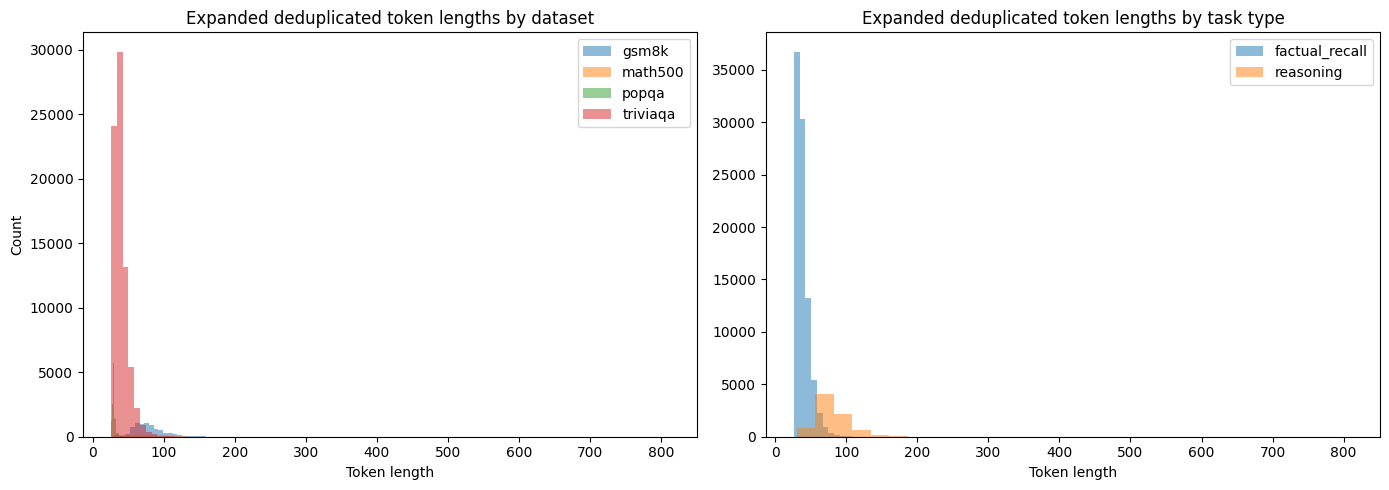
\includegraphics[width=0.95\textwidth]{figures/expanded_lengths_before_deduped.png}
    \caption{Token-length distributions before expanded matching. The
    factual-recall pool is concentrated at substantially shorter token
    lengths, while reasoning examples have a much longer tail.}
    \label{fig:expanded-lengths-before}
\end{figure}

\begin{figure}[H]
    \centering
    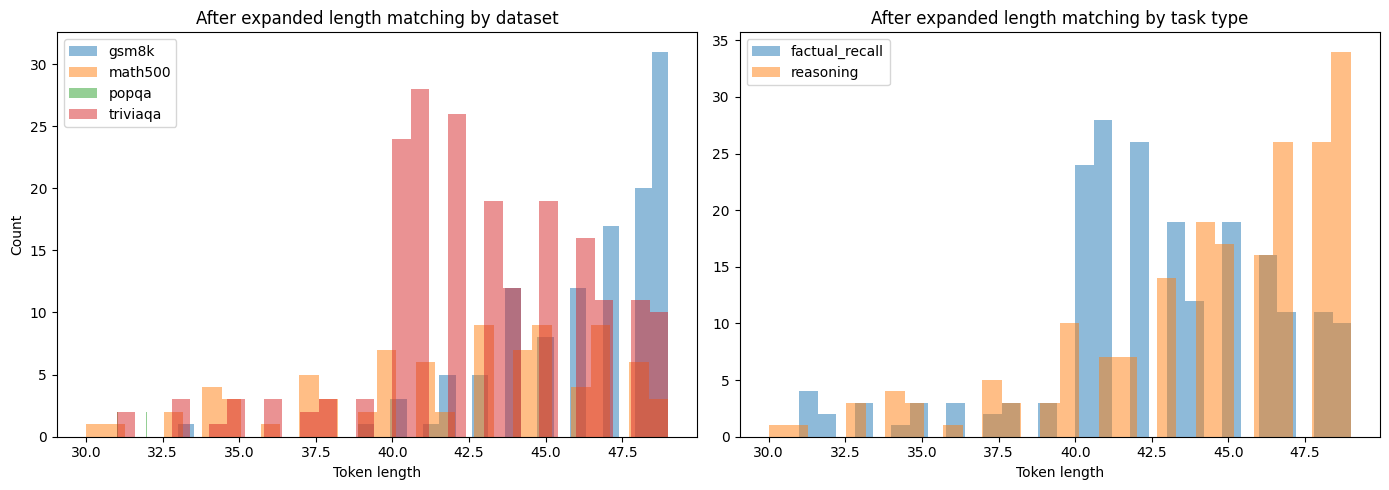
\includegraphics[width=0.95\textwidth]{figures/expanded_lengths_after_matching.png}
    \caption{Token-length distributions after expanded matching. The
    two task groups overlap much more strongly, although reasoning
    remains slightly shifted toward longer prompts.}
    \label{fig:expanded-lengths-after}
\end{figure}

\paragraph{Surface baselines.}

The length-only baseline is substantially weaker than in the original
experiment:

\[
\mathrm{Accuracy}=0.6475 \pm 0.0533,
\qquad
\mathrm{AUROC}=0.6645 \pm 0.0585.
\]

However, a TF--IDF lexical baseline remains very strong:

\[
\mathrm{Accuracy}=0.9600 \pm 0.0146,
\qquad
\mathrm{AUROC}=0.9911 \pm 0.0113.
\]

This indicates that lexical and domain differences between the current
reasoning-oriented and factual-recall pools remain highly predictive,
even after length control.

\paragraph{Representation extraction.}

For the 400 matched examples, we extract hidden states using the
existing custom Qwen3-0.6B implementation and tokenizer. No tokens are
generated. For each formatted prompt, the model returns

\[
H_i \in \mathbb{R}^{28 \times 1024}.
\]

The saved tensors have shapes

\[
H \in \mathbb{R}^{400 \times 28 \times 1024},
\qquad
X^{(28)} \in \mathbb{R}^{400 \times 1024}.
\]

The primary analysis uses the final-layer prompt-token representation
\(X^{(28)}\).

\paragraph{PCA.}

PCA is fit to \(X^{(28)}\) without labels. The first two components
explain

\[
\mathrm{Var}(PC1)=21.97\%,
\qquad
\mathrm{Var}(PC2)=12.25\%,
\]

for a combined explained variance of 34.22\%.

\begin{figure}[H]
    \centering
    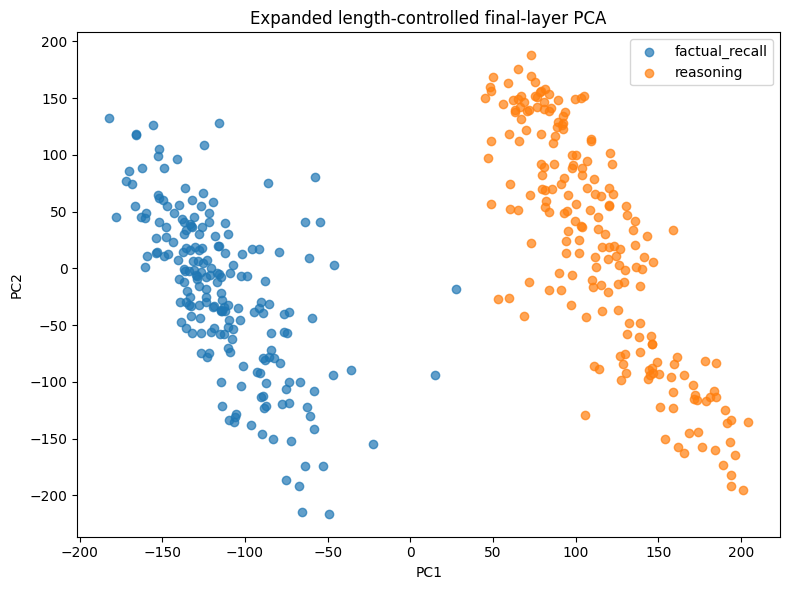
\includegraphics[width=0.75\textwidth]{figures/expanded_final_layer_pca.png}
    \caption{Final-layer PCA for the expanded length-controlled
    dataset. Labels are used only for visualization after PCA fitting.
    The two task groups separate strongly along the dominant principal
    components, but this should not be interpreted as proof that PC1 is
    a reasoning direction.}
    \label{fig:expanded-pca}
\end{figure}

\paragraph{Final-layer linear probe.}

A 5-fold logistic-regression probe on Qwen final-layer representations
achieves

\[
\mathrm{Accuracy}=0.9975 \pm 0.0050,
\qquad
\mathrm{Balanced\ Accuracy}=0.9975 \pm 0.0050,
\qquad
\mathrm{AUROC}=1.0000 \pm 0.0000.
\]

A repeated random-label control over 10 shuffles returns to chance:

\[
\mathrm{Accuracy}=0.4875 \pm 0.0360,
\qquad
\mathrm{AUROC}=0.4816 \pm 0.0453.
\]

\paragraph{Cross-dataset evaluation.}

We also test whether the final-layer probe transfers across source
datasets. Training on MATH-500 and PopQA and testing on GSM8K and
TriviaQA gives 0.939 accuracy, 0.952 balanced accuracy, and 0.999
AUROC. Reversing the direction gives 0.966 accuracy, 0.982 balanced
accuracy, and 1.000 AUROC.

These results are promising, but the first split contains only four
PopQA examples in the training set and the reverse split contains only
four PopQA examples in the test set. Therefore, these cross-source
results should be interpreted cautiously.

\paragraph{Per-dataset probes and multi-seed robustness.}

MATH-500 versus TriviaQA achieves \(0.9929 \pm 0.0087\) accuracy and
1.000 AUROC. GSM8K versus TriviaQA achieves perfect accuracy and AUROC.
MATH-500 versus PopQA and GSM8K versus PopQA are skipped because only
four PopQA examples remain in the matched dataset.

Repeating the main final-layer probe with seeds 42, 123, and 456 gives
identical mean performance: \(0.9975\) accuracy and 1.000 AUROC.

\paragraph{Summary comparison.}

\begin{table}[H]
    \centering
    \begin{tabular}{lcc}
        \toprule
        Method & Accuracy & AUROC \\
        \midrule
        Length-only & \(0.6475 \pm 0.0533\) & \(0.6645 \pm 0.0585\) \\
        TF--IDF lexical & \(0.9600 \pm 0.0146\) & \(0.9911 \pm 0.0113\) \\
        Qwen final-layer probe & \(0.9975 \pm 0.0050\) & \(1.0000 \pm 0.0000\) \\
        Random-label probe & \(0.4875 \pm 0.0360\) & \(0.4816 \pm 0.0453\) \\
        \bottomrule
    \end{tabular}
    \caption{Expanded RQ1 baseline and representation-probe comparison.}
    \label{tab:expanded-baseline-summary}
\end{table}

\paragraph{Interpretation.}

The expanded experiment substantially improves over the strict
20-example length-matched control. It shows that Qwen3-0.6B
final-layer representations robustly distinguish the current
reasoning-oriented and factual-recall task groups after distributional
length matching. However, the TF--IDF baseline demonstrates that
lexical and domain cues remain strong. Therefore, the result supports
representation-level task-group separability, but not yet an intrinsic
or single-direction account of reasoning.

% ------------------------------------------------------------

% ------------------------------------------------------------

\subsubsection{Final Single-Direction Experiment}

The final RQ1 experiment directly tests whether the expanded reasoning-oriented versus factual-recall separation can be captured by one direction per transformer layer. We use the previously extracted hidden-state tensor
\[
H \in \mathbb{R}^{400 \times 28 \times 1024},
\]
where each row corresponds to the final formatted prompt-token representation after each transformer block.

For each layer \(l\), we evaluate three held-out methods under 5-fold stratified cross-validation. First, the mean-difference direction is computed from training data only:
\[
d_{\mathrm{mean}}^{(l)} = \mu_R^{(l)} - \mu_F^{(l)}.
\]
Second, we train a logistic-regression probe on training examples and use the normalized weight vector as a single direction:
\[
d_{\mathrm{probe}}^{(l)} = \frac{w^{(l)}}{\|w^{(l)}\|_2}.
\]
Third, both one-dimensional methods are compared to the standard full 1024-D logistic-regression probe.

\paragraph{Main results.}
The best mean-difference direction occurs at layer 18 and achieves
\[
\mathrm{Accuracy}=0.9975 \pm 0.0050,\quad
\mathrm{Balanced\ Accuracy}=0.9975 \pm 0.0050,\quad
\mathrm{AUROC}=1.0000 \pm 0.0000.
\]
The best probe-weight direction occurs at layer 12 and achieves the same performance. The best full 1024-D linear probe also occurs at layer 12 and achieves the same accuracy and AUROC.

\begin{table}[H]
    \centering
    \begin{tabular}{lcc}
        \toprule
        Method & Accuracy & AUROC \\
        \midrule
        Length-only & \(0.6475 \pm 0.0533\) & \(0.6645 \pm 0.0585\) \\
        TF--IDF lexical & \(0.9600 \pm 0.0146\) & \(0.9911 \pm 0.0113\) \\
        Mean-difference direction, layer 18 & \(0.9975 \pm 0.0050\) & \(1.0000 \pm 0.0000\) \\
        Probe-weight direction, layer 12 & \(0.9975 \pm 0.0050\) & \(1.0000 \pm 0.0000\) \\
        Full 1024-D linear probe, layer 12 & \(0.9975 \pm 0.0050\) & \(1.0000 \pm 0.0000\) \\
        Random-label control & \(0.4875 \pm 0.0360\) & \(0.4816 \pm 0.0453\) \\
        \bottomrule
    \end{tabular}
    \caption{Final RQ1 comparison between surface baselines, single-direction methods, the full 1024-D probe, and the random-label control.}
    \label{tab:rq1-final-baseline-comparison}
\end{table}

\paragraph{Layer-wise behavior.}
Both one-dimensional directions perform strongly across all 28 layers. The mean-difference direction begins with AUROC 0.9924 at layer 1 and reaches perfect AUROC from layer 18 onward. The probe-weight direction begins with AUROC 0.9944 at layer 1 and reaches perfect AUROC by layer 12.

\begin{figure}[H]
    \centering
    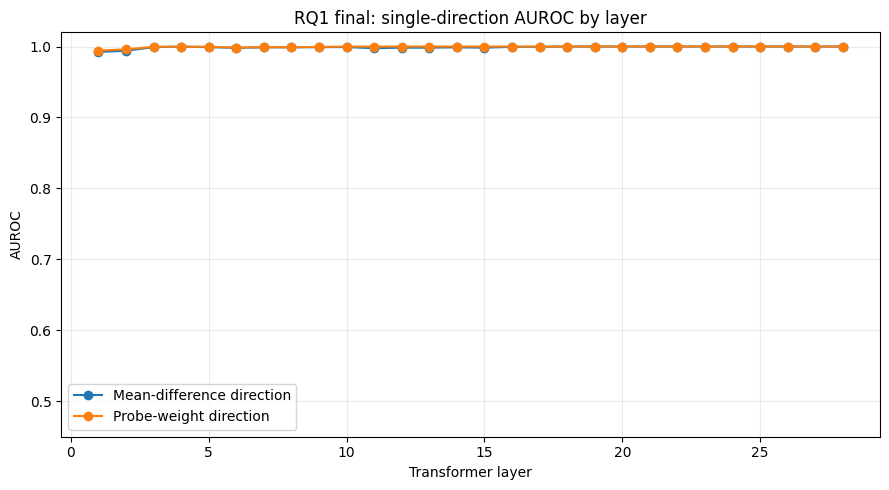
\includegraphics[width=0.85\textwidth]{figures/rq1_final/layerwise_auroc.png}
    \caption{Single-direction AUROC across transformer layers.}
    \label{fig:rq1-layerwise-auroc}
\end{figure}

\begin{figure}[H]
    \centering
    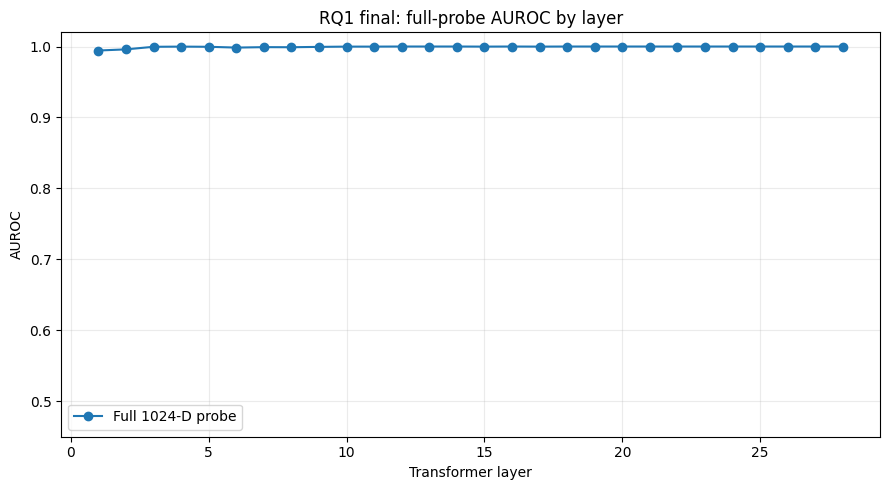
\includegraphics[width=0.85\textwidth]{figures/rq1_final/full_probe_auroc.png}
    \caption{Full 1024-D linear-probe AUROC across transformer layers.}
    \label{fig:rq1-full-probe-auroc}
\end{figure}

\begin{figure}[H]
    \centering
    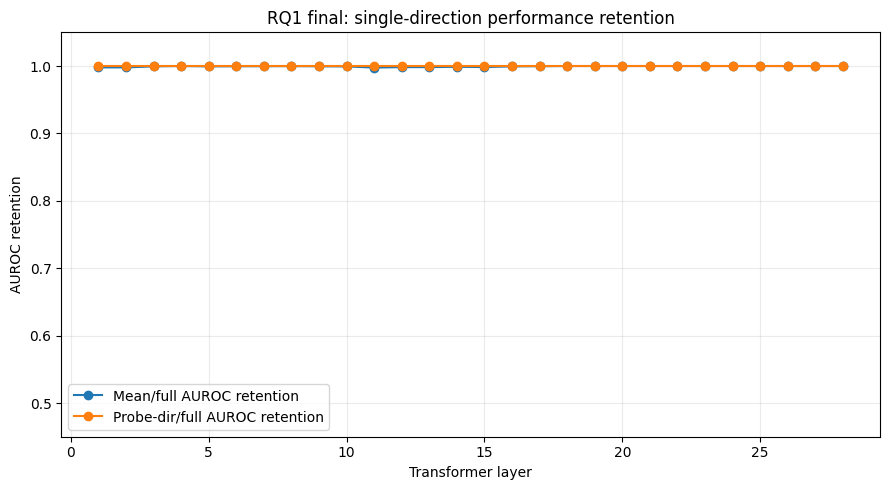
\includegraphics[width=0.85\textwidth]{figures/rq1_final/performance_retention.png}
    \caption{AUROC retention of one-dimensional directions relative to the full 1024-D probe. Retention is essentially 1.0 across layers.}
    \label{fig:rq1-performance-retention}
\end{figure}

\paragraph{Direction alignment.}
The average cosine similarity between \(d_{\mathrm{mean}}\) and \(d_{\mathrm{probe}}\) across layers is 0.8495. Alignment is very high in early layers, decreases in middle layers, and rises again in later layers.

\begin{figure}[H]
    \centering
    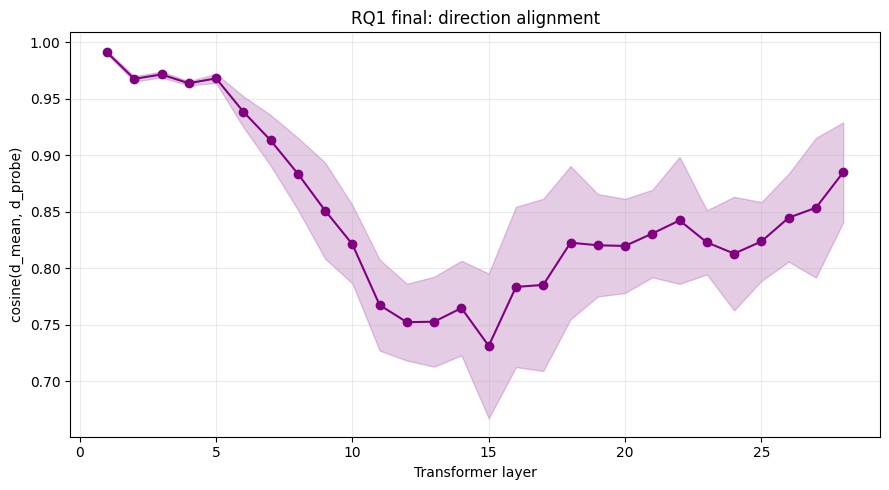
\includegraphics[width=0.85\textwidth]{figures/rq1_final/direction_alignment.png}
    \caption{Cosine alignment between the mean-difference direction and probe-weight direction across layers.}
    \label{fig:rq1-direction-alignment}
\end{figure}

\paragraph{Held-out score distributions.}
For the best mean-difference layer, layer 18, the held-out projected scores are almost disjoint. Factual-recall examples have mean score \(-19.73\), while reasoning-oriented examples have mean score \(19.73\). The absolute score separation is 39.46, and the overlap interval width is only 0.0675.

\begin{figure}[H]
    \centering
    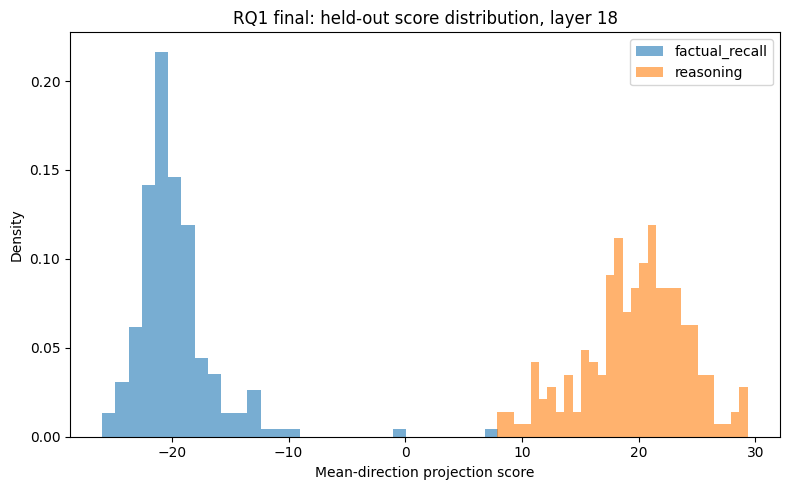
\includegraphics[width=0.75\textwidth]{figures/rq1_final/score_distribution_best_layer.png}
    \caption{Held-out score distributions after projecting layer-18 representations onto the mean-difference direction.}
    \label{fig:rq1-score-distribution}
\end{figure}

\paragraph{Final RQ1 decision.}
The final decision is \textbf{strong support}: the evidence supports a low-dimensional, approximately single-direction separation between the studied reasoning-oriented and factual-recall task groups. This does not show that the direction is causal, that it is an intrinsic reasoning mechanism, or that factual recall is experimentally identical to memorization. The strong TF--IDF baseline remains a major limitation.

\subsubsection{Multi-Dataset Evaluation}

Length matching alone cannot remove dataset identity, lexical, or
domain confounds.

We therefore plan to construct reasoning and memorization collections
using multiple source datasets per behavioral category.

The purpose is to avoid the mapping

\[
\text{dataset identity}
\equiv
\text{behavioral label}.
\]

All datasets will use a common prompt-formatting pipeline and will be
analyzed for token-length and surface-feature differences.

% ------------------------------------------------------------

\subsubsection{Surface-Feature Baselines}

To quantify how easily the behavioral labels can be predicted without
access to model representations, we include simple baselines such as:

\begin{itemize}

    \item token length;

    \item lexical / bag-of-words features;

    \item TF--IDF representations;

    \item and other simple prompt-level statistics where appropriate.

\end{itemize}

A representation-based classifier should be interpreted cautiously
when similarly strong classification can be obtained from trivial
surface features.

% ------------------------------------------------------------

\subsubsection{Cross-Dataset Generalization}

Random cross-validation evaluates generalization to unseen examples
from the same source datasets, but does not eliminate dataset-specific
signals.

A stronger experiment trains a probe using some reasoning and
memorization datasets and evaluates it on held-out source datasets.

Conceptually,

\[
\mathcal{D}^{\mathrm{train}}_R
\cap
\mathcal{D}^{\mathrm{test}}_R
=
\emptyset
\]

and

\[
\mathcal{D}^{\mathrm{train}}_M
\cap
\mathcal{D}^{\mathrm{test}}_M
=
\emptyset
\]

at the dataset-source level.

If a linear direction generalizes to unseen reasoning and memorization
datasets, this provides substantially stronger evidence that the
learned geometry captures a transferable behavioral distinction rather
than dataset identity.

% ============================================================

\subsection{Explicit Single-Direction Test}

Only after establishing that representation-level separation survives
the major confound controls do we directly test the
single-direction hypothesis.

Using training examples, we construct

\[
d^{(l)}
=
\mu_R^{(l)}
-
\mu_M^{(l)},
\]

where

\[
\mu_R^{(l)}
=
\frac{1}{N_R}
\sum_i h_{R,i}^{(l)}
\]

and

\[
\mu_M^{(l)}
=
\frac{1}{N_M}
\sum_i h_{M,i}^{(l)}.
\]

The normalized direction is

\[
\hat{d}^{(l)}
=
\frac{d^{(l)}}{\|d^{(l)}\|_2}.
\]

Held-out representations are projected onto this single direction:

\[
s_i
=
(h_i-\mu_{\mathrm{train}})^\top
\hat{d}^{(l)}.
\]

This converts each 1024-dimensional representation into a single
scalar coordinate.

We then evaluate how much reasoning--memorization information remains
in this one-dimensional projection.

% ============================================================

\subsection{Single Direction Versus Multidimensional Structure}

Linear separability does not imply that one fixed direction provides
an adequate description of the underlying geometry.

We therefore compare:

\begin{enumerate}

    \item performance using a single explicit direction;

    \item performance using several representation directions;

    \item and performance using the complete linear representation
    space.

\end{enumerate}

If one direction achieves performance comparable to richer
representations, this supports a low-dimensional or
single-direction description.

If performance increases substantially as additional dimensions are
introduced, this provides evidence that the reasoning--memorization
distinction is better described by a multidimensional subspace.

% ============================================================

\subsection{Layer-wise Analysis}

The initial diagnostic experiments analyze only the final transformer
layer.

After establishing a controlled dataset and evaluation protocol, the
same analyses will be applied independently across all 28 transformer
layers.

For each layer \(l\), we will measure:

\begin{itemize}

    \item PCA geometry;

    \item linear-probe performance;

    \item single-direction performance;

    \item dimensionality--performance relationships;

    \item and representation/subspace similarity.

\end{itemize}

This will allow us to determine where reasoning--memorization
structure emerges and how its geometry changes through transformer
depth.

% ============================================================

\subsection{Extraction-Position Ablation}

The primary representation currently corresponds to the final token
of the formatted model input.

To determine whether the observed geometry depends on this choice, we
will compare it against representations extracted from the final
semantic token of the original user prompt.

This provides an explicit test of sensitivity to chat-template and
assistant-prefix positions.

% ============================================================


\subsection{Current RQ1 Status}

RQ1 is now closed. The final experiment directly tests whether the expanded task-group separation can be captured by one direction per layer. Under held-out 5-fold cross-validation, both the mean-difference direction and the probe-weight direction reach \(1.0000 \pm 0.0000\) AUROC, matching the full 1024-D linear probe. The best mean-difference layer is layer 18, and the best probe-weight layer is layer 12.

This provides strong support for an approximately single-direction separation between the studied reasoning-oriented and factual-recall task groups in Qwen3-0.6B hidden representations. However, the strong TF--IDF baseline means lexical and domain cues remain a serious limitation. Therefore, we do not claim that the direction is a causal mechanism or an intrinsic representation of reasoning itself.

\section{RQ2: Representation Evolution During Reinforcement Learning}\section{RQ2: Representation Evolution During Reinforcement Learning}

We study how reasoning and memorization representations evolve
throughout reinforcement learning, comparing representations extracted
from multiple RL checkpoints rather than only the final model.

\subsection{Setup}

\begin{itemize}

    \item RL algorithm: GRPO
    \item Training checkpoints
    \item Hyperparameters
    \item Reward function

\end{itemize}

\subsection{Method}

\begin{itemize}

    \item Hidden-state extraction across checkpoints
    \item Representation drift
    \item Cosine similarity
    \item Centered Kernel Alignment (CKA)
    \item Subspace similarity

\end{itemize}

\subsection{Results}

% Experiments pending.

% ============================================================

\section{RQ3: Cross-Task Generalization}

We investigate whether representational structures identified on one
set of reasoning and memorization tasks generalize to other domains.

\subsection{Setup}

\begin{itemize}

    \item Multiple reasoning datasets
    \item Multiple factual-recall / memorization datasets
    \item Held-out source-dataset evaluation
    \item Controlled prompt formatting and length analysis

\end{itemize}

\subsection{Method}

\begin{itemize}

    \item Cross-dataset linear probing
    \item Direction transfer
    \item Representation similarity
    \item PCA
    \item Subspace analysis

\end{itemize}

\subsection{Results}

% Experiments pending.

% ============================================================

\section{RQ4: Mechanistic Structure}

Finally, we investigate whether reasoning and memorization
representations can be decomposed into multiple interpretable latent
features.

\subsection{Setup}

\begin{itemize}

    \item Sparse autoencoder training details
    \item Dictionary size
    \item Sparsity coefficient
    \item Target transformer layers

\end{itemize}

\subsection{Method}

\begin{itemize}

    \item Sparse Autoencoders
    \item Feature activation analysis
    \item Layer-wise comparison
    \item Feature evolution during reinforcement learning

\end{itemize}

\subsection{Results}

% Experiments pending.

% ============================================================


\section{Discussion}

The RQ1 experiments show why representation probing must be paired with increasingly strong controls. The original MATH-500 versus PopQA comparison produced perfect hidden-state separability, but token length alone nearly solved the same classification problem. The expanded 400-example experiment reduced length as a dominant confound, but TF--IDF lexical features remained highly predictive.

The final single-direction experiment answers the narrower geometric question directly. Given the current controlled task groups, the separation in Qwen3-0.6B representations is not merely linearly decodable in 1024 dimensions; it is almost completely captured by one scalar projection. Both a simple class-mean direction and a normalized probe-weight direction match the full linear probe, with perfect AUROC at their best layers and near-perfect performance across depth.

The correct interpretation is therefore strong but bounded. RQ1 supports an approximately single-direction separation between the studied reasoning-oriented and factual-recall task groups. It does not establish that this direction is a causal reasoning mechanism, nor that factual recall is the same as memorization. The lexical baseline shows that task/domain wording remains a major confound.

\section{Limitations}

Current limitations include:

\begin{itemize}
    \item experiments currently focus on Qwen3-0.6B;
    \item the primary extraction position is the final formatted-prompt token;
    \item the expanded matched dataset is balanced by task group but not by source dataset;
    \item PopQA contributes only four examples after matching;
    \item TF--IDF lexical features remain highly predictive, indicating strong lexical/domain confounding;
    \item the result supports a task-group separation direction, not a causal reasoning mechanism;
    \item factual recall is not experimentally equivalent to memorization;
    \item larger-model and stronger semantic-control validation remain future work outside RQ1.
\end{itemize}

\section{Related Work}\section{Related Work}

% Reasoning Models
%
% Reasoning vs. Memorization
%
% Direction-based representation analysis
%
% Representation probing
%
% Dataset confounding in probing
%
% Reinforcement Learning for LLMs
%
% Mechanistic Interpretability
%
% Sparse Autoencoders

% ============================================================

\section{Broader Impact and Ethics Statement}

% Dual-use considerations of interpretability tooling,
% implications of identifying/steering reasoning vs. memorization
% representations, and data licensing for benchmarks used.

% ============================================================

\section{Reproducibility Statement}

For each experiment, we plan to release:

\begin{itemize}

    \item dataset preprocessing and sampling scripts;

    \item dataset-source metadata;

    \item prompt-length statistics;

    \item model and tokenizer configuration;

    \item exact prompt templates;

    \item representation extraction code;

    \item extraction-position definitions;

    \item random seeds;

    \item probing and representation-analysis scripts;

    \item baseline classifiers;

    \item reinforcement-learning configurations;

    \item and scripts reproducing figures and tables.

\end{itemize}

Extracted representation artifacts additionally retain sample metadata
and the configuration describing how each representation was obtained.

% ============================================================


\section{Conclusion}

RQ1 asked whether reasoning-oriented and factual-recall representations in Qwen3-0.6B can be separated by a single linear direction. The final answer is yes for the current controlled task groups: both a mean-difference direction and a normalized probe-weight direction match the full 1024-D linear probe under held-out cross-validation. The best single-direction AUROC is 1.0000, the best full-probe AUROC is 1.0000, and the performance gap is 0.0000.

This closes RQ1 with strong support for an approximately single-direction geometric separation. The result should not be overstated. Because TF--IDF lexical features also classify the task groups very strongly, the identified direction may reflect a mixture of task type, lexical style, domain, and dataset identity. The paper therefore frames the result as a single-direction separation of the studied task groups, not as proof of an intrinsic or causal reasoning axis.

\bibliographystyle\bibliographystyle{plain}
\bibliography{references}

% ============================================================

\appendix

\section{Full Hyperparameters}

% ============================================================

\section{Representation Extraction Details}

% Exact prompt formatting
% Tokenization
% Extraction position
% Hidden-state boundary
% Model configuration

% ============================================================

\section{Dataset Diagnostics}

This appendix records the current dataset diagnostics for RQ1.

\subsection{Original Diagnostic Dataset}

The original diagnostic dataset contains 100 MATH-500 examples labeled
as reasoning and 100 PopQA examples labeled as memorization. Source
dataset and behavioral label are perfectly correlated in this setup.

The original length-only baseline achieves approximately 0.965
accuracy and 0.994 AUROC, showing that token length is a strong scalar
confound.

\subsection{Length-Matched Dataset}

The length-matched dataset is constructed using one-to-one matching
without replacement and tolerance \(\delta=5\). The resulting subset
contains 10 matched reasoning examples and 10 matched memorization
examples.

\begin{table}[H]
    \centering
    \begin{tabular}{lcc}
        \toprule
        Quantity & Reasoning & Memorization \\
        \midrule
        Matched examples & 10 & 10 \\
        Hidden-state tensor shape & \(10 \times 28 \times 1024\) &
        \(10 \times 28 \times 1024\) \\
        Final-layer matrix shape & \(10 \times 1024\) &
        \(10 \times 1024\) \\
        Mean token length & 28.1 & 25.1 \\
        Median token length & 29.0 & 24.5 \\
        Minimum token length & 22 & 22 \\
        Maximum token length & 32 & 29 \\
        \bottomrule
    \end{tabular}
    \caption{
    Length-matched dataset diagnostics for the first controlled RQ1
    experiment.
    }
    \label{tab:appendix-length-matched-diagnostics}
\end{table}

\subsection{Controlled Baselines}

\begin{table}[H]
    \centering
    \begin{tabular}{lccc}
        \toprule
        Experiment & Accuracy & Balanced Accuracy & AUROC \\
        \midrule
        Length-only baseline &
        \(0.600 \pm 0.122\) &
        \(0.600 \pm 0.122\) &
        \(0.875 \pm 0.194\) \\
        Hidden-state probe &
        \(1.000 \pm 0.000\) &
        \(1.000 \pm 0.000\) &
        \(1.000 \pm 0.000\) \\
        Random-label control &
        \(0.400 \pm 0.255\) &
        \(0.400 \pm 0.255\) &
        \(0.500 \pm 0.316\) \\
        \bottomrule
    \end{tabular}
    \caption{
    Five-fold stratified cross-validation results on the
    length-matched subset.
    }
    \label{tab:appendix-controlled-baselines}
\end{table}


\subsection{Expanded Multi-Dataset Control}

The expanded RQ1 control uses MATH-500, GSM8K, PopQA, and TriviaQA.
The raw pool contains 160,624 examples; after deduplication, 97,477
examples remain. Distributional length matching produces 200
reasoning-oriented and 200 factual-recall examples.

\begin{table}[H]
    \centering
    \begin{tabular}{lccc}
        \toprule
        Source & Raw count & Deduplicated count & Matched count \\
        \midrule
        MATH-500 & 500 & 500 & 84 \\
        GSM8K & 7473 & 7473 & 116 \\
        PopQA & 14267 & 13066 & 4 \\
        TriviaQA & 138384 & 76438 & 196 \\
        \bottomrule
    \end{tabular}
    \caption{Expanded dataset counts before and after deduplication and matching.}
    \label{tab:appendix-expanded-counts}
\end{table}

\begin{table}[H]
    \centering
    \begin{tabular}{lccc}
        \toprule
        Experiment & Accuracy & Balanced Accuracy & AUROC \\
        \midrule
        Length-only baseline &
        \(0.6475 \pm 0.0533\) &
        \(0.6475 \pm 0.0533\) &
        \(0.6645 \pm 0.0585\) \\
        TF--IDF lexical baseline &
        \(0.9600 \pm 0.0146\) &
        \(0.9600 \pm 0.0146\) &
        \(0.9911 \pm 0.0113\) \\
        Qwen final-layer probe &
        \(0.9975 \pm 0.0050\) &
        \(0.9975 \pm 0.0050\) &
        \(1.0000 \pm 0.0000\) \\
        Random-label probe &
        \(0.4875 \pm 0.0360\) &
        \(0.4875 \pm 0.0360\) &
        \(0.4816 \pm 0.0453\) \\
        \bottomrule
    \end{tabular}
    \caption{Expanded RQ1 control baselines and final-layer probe results.}
    \label{tab:appendix-expanded-baselines}
\end{table}

% ============================================================

\subsection{Final RQ1 Single-Direction Results}

\begin{table}[H]
    \centering
    \begin{tabular}{lcc}
        \toprule
        Result & Layer & AUROC \\
        \midrule
        Best mean-difference direction & 18 & \(1.0000 \pm 0.0000\) \\
        Best probe-weight direction & 12 & \(1.0000 \pm 0.0000\) \\
        Best full 1024-D probe & 12 & \(1.0000 \pm 0.0000\) \\
        \bottomrule
    \end{tabular}
    \caption{Best-layer final RQ1 results.}
    \label{tab:appendix-rq1-final-best}
\end{table}

\section{Additional Per-Layer Results}

% Per-layer PCA
% Probe performance
% Single-direction performance
% Direction projections
% Additional ablations

% ============================================================

\section{Extended Related Work}

\end{document}
